\documentclass[letterpaper]{article}
\usepackage{aaai24}
% \usepackage[submission]{aaai24}

\usepackage{booktabs} % For formal tables
% \usepackage{float}
\usepackage{caption}
\usepackage{multirow}
\usepackage{amsmath}
\usepackage{amsfonts}
\setcounter{secnumdepth}{2}

\captionsetup[table]{font=footnotesize}
\captionsetup[figure]{font=footnotesize}
% \usepackage{subcaption}
\usepackage{etoc}

\usepackage{times} % DO NOT CHANGE THIS
\usepackage{helvet} % DO NOT CHANGE THIS
\usepackage{courier} % DO NOT CHANGE THIS
\usepackage[hyphens]{url} % DO NOT CHANGE THIS
\usepackage{graphicx} % DO NOT CHANGE THIS
\urlstyle{rm} % DO NOT CHANGE THIS
\def\UrlFont{\rm} % DO NOT CHANGE THIS
\usepackage{graphicx} % DO NOT CHANGE THIS
\usepackage{natbib} % DO NOT CHANGE THIS
\usepackage{caption} % DO NOT CHANGE THIS
\frenchspacing % DO NOT CHANGE THIS
\setlength{\pdfpagewidth}{8.5in} % DO NOT CHANGE THIS
\setlength{\pdfpageheight}{11in} % DO NOT CHANGE THIS
%
% Keep the \pdfinfo as shown here. There’s no need
% for you to add the /Title and /Author tags.
\pdfinfo{
/TemplateVersion (2024.1)
}

\title{Advancing Ante-Hoc Explainable Models through Generative Adversarial Networks}
\author {
    % Authors
    Tanmay Garg,
    Deepika Vemuri,
    Vineeth N Balasubramanian
}
\affiliations {
    % Affiliations
    Indian Institute of Technology, Hyderabad, India\\
    gargtanmay1@gmail.com, ai22resch11001@iith.ac.in, vineethnb@cse.iith.ac.in
}

\begin{document}
\maketitle



\begin{abstract}

This paper presents a novel concept learning framework for enhancing model interpretability and performance in visual classification tasks. Our approach appends an unsupervised explanation generator to the primary classifier network and makes use of adversarial training. During training, the explanation module is optimized to extract visual concepts from the classifier's latent representations, while the GAN-based module aims to discriminate images generated from concepts, from true images. This joint training scheme enables the model to implicitly align its internally learned concepts with human-interpretable visual properties. Comprehensive experiments demonstrate the robustness of our approach, while producing coherent concept activations. We analyse the learned concepts, showing their semantic concordance with object parts and visual attributes. We also study how perturbations in the adversarial training protocol impact both classification and concept acquisition.
In summary, this work presents a significant step towards building inherently interpretable deep vision models with task-aligned concept representations - a key enabler for developing trustworthy AI for real-world perception tasks.

\end{abstract}



\maketitle
\section{Introduction}\label{sec:intro}

Deep neural networks (DNNs) have ushered in a revolution across domains like Computer Vision \cite{VGG}, Natural Language Processing \cite{gpt3}, Healthcare \cite{health}, and Finance \cite{finance}. They have made significant strides in handling intricate tasks like image recognition, machine translation, and anomaly detection. However, they come with a challenge - they are essentially black-box systems. The increasing complexity of these models has led to a lack of transparency and interpretability \cite{lipton, ravikumar}. This opacity has raised significant concerns within the scientific community, particularly in critical areas like healthcare and criminal justice. In healthcare, for instance, patients would want to know why a disease-diagnosing model provided them with a certain result.
%In healthcare, for instance, it's crucial for patients to understand why a disease-diagnosing model provides a specific result. 
Additionally, being able to identify and verify false positives and negatives is essential, as such oversight could have potentially serious consequences.

Explainable models have become instrumental in establishing transparency, a key factor in building trust with users. 
%Their emergence has brought about a fresh perspective to the explainability of Deep Neural Networks (DNNs). 
In recent years, there has been a surge of research in this area, with most works coming under two broad categories: post-hoc and ante-hoc methods.

\textit{Post-hoc explainability} methods attempt to provide explanations as a separate module on already trained models.
Saliency maps \cite{saliency_maps} are a prime example of this line of work, introducing a method that visually highlights the points on an image that activate neurons, depending on the predicted class by the deep neural network.  However, decoupling the explanation method from the explained model makes it a challenge to discern whether the model's prediction was incorrect or the explanation provided was at fault.

\textit{Ante-hoc explainability} methods, on the other hand, provide explanations implicitly during model training itself. There have been several ante-hoc works in recent times that make use of \textit{concepts} \cite{CBM, efros, efros2}. These methods assume that each class can be broken down into a set of concepts, i.e. that concepts can be used to signify the distinctive features or characteristics that make up a particular class. For example, in the case of MNIST \cite{MNSIT}, concepts could include straight lines, types of curves in the digits, or even more specific patterns that may appear in a digit. 
Self-explaining neural networks (SENN) \cite{SENN} exemplify such approaches, offering a straightforward means to acquire interpretable concepts by extending a linear predictor. When presented with an input image, the prediction is generated based on a weighted combination of these concepts. 
\cite{Sarkar2021AFF} introduce a method to account for varying degrees of concept supervision in a SENN-like framework. 


In this paper, we build upon and extend the findings of \cite{Sarkar2021AFF}, showing how introducing an adversarial component into the framework can better guide representation learning. We propose a modified loss, harness the benefits of randomization and use labels as supplementary information for conditioning the reconstruction process.

\begin{figure*}[h!]
    \centering
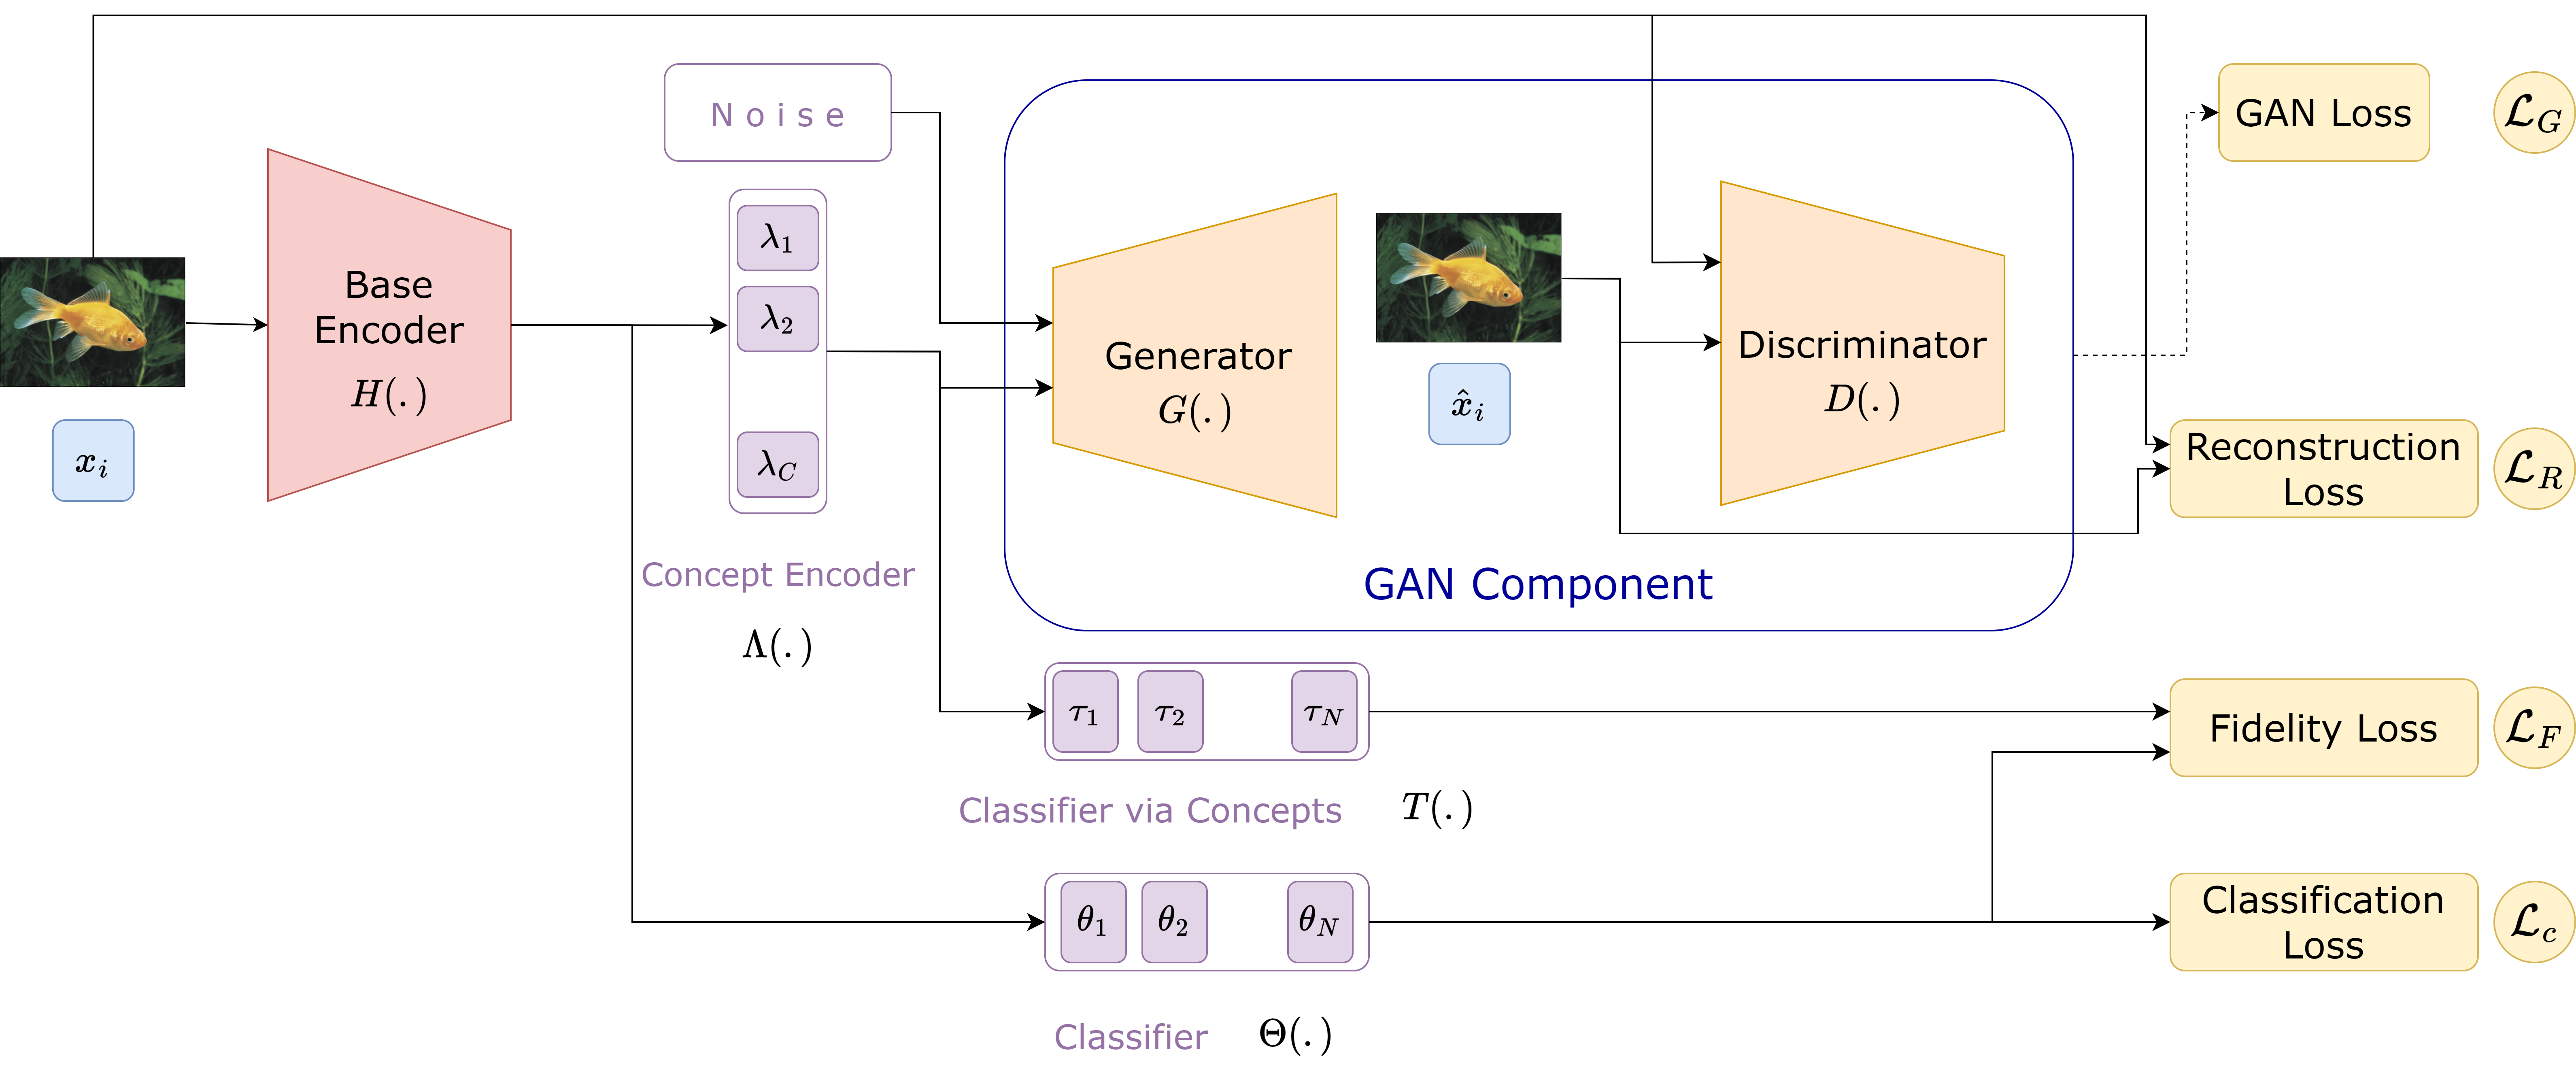
\includegraphics[width=1.8\columnwidth]{images/senndiag.png}
    \caption{Overview of our Proposed Architecture. N is the number of classes, C is the number of concepts}
    \label{fig:senn_gan}
\end{figure*}

To summarize, our contributions are as follows:
\begin{itemize}
    \item We introduce a novel, enhanced architecture that demonstrates improved performance compared to the baselines. The key aspect here lies in the integration of a Generative Adversarial Network (GAN) \cite{GAN} within the architecture.
    \item We conduct a series of experiments to analyze and compare the impact of different GAN variants, such as a vanilla GAN \cite{GAN} and conditional GAN (cGAN) \cite{CGAN}, on performance and concept visualization.
    \item We explore various methods for generating noise to understand how noise sampled from a Gaussian distribution influences concept generation in our framework.
    \item Our approach capitalizes on the adversarial nature of GANs and noise generation method to produce higher-quality images that facilitate more robust concept encoding.
\end{itemize}

\section{Methodology}\label{sec:method}
\subsection{Background}\label{sec:background}


\textbf{Self Explaining Neural Networks \cite{SENN}:} This was one of the first works to propose a robust ante-hoc framework along with metrics to measure interpretability. Starting with a simple linear regression model, which is inherently interpretable - given that the model's parameters are linearly related, the paper successively generalizes it to more complicated models like neural networks. Their key goals were for concepts to retain image information, to be distinct between classes, and to be  understandable to humans. To address these goals, an autoencoder encodes images into concepts optimized using reconstruction and classification losses. One limitation we observe is that the concepts are derived solely from the dataset without leveraging additional information like labels or extra images. Extensions to this attempt to enhance concept explainability through disentanglement and contrastive learning \cite{CSENN}. Our work leverages generative models to create more refined concepts that address some of the original limitations.

\textbf{Ante-Hoc Explainability via Concepts \cite{Sarkar2021AFF}:} In this work, an ante-hoc framework, allowing for different levels of supervision, including fully supervised and unsupervised concept learning, was proposed, building upon \cite{SENN}. 
The framework could be added to any existing backbone model and optimized jointly. The paper primarily introduces the notion of \textit{fidelity loss} and a way to visualize the concepts learnt by the model. 
In our work, we assume the basic setup from this paper and make specific modifications to enhance it.

\subsection{Proposed Architecture}\label{sec:arch}
A typical deep learning classification pipeline has a base encoder function followed by a classifier function. Let $\mathcal{X}$ be the input space and $\mathcal{Y}$ be the label space for our training set $\mathcal{D} = \{x_i, y_i\}_{i=1}^N$, sampled iid from some source distribution $\mathcal{P} : \mathcal{X} \times\mathcal{Y}$, where $\mathcal{X} \in \mathrm{R}^d$, and $\mathcal{Y}$ is a one-hot encoded vector. The base encoder $H(.)$ extracts representation vectors that are then fed into the classifier $\Theta(.)$. One way of making such a setup interpretable is to provide explanations via concepts. In order to do this, a concept encoder $\Lambda(.)$ is introduced in the pipeline. $\Lambda(.)$ takes in the representations extracted by $H(.)$ and learns a set of concepts $\{\lambda_1, \lambda_2,…\lambda_C\}$ that are used to explain the classification by passing them through $T(.)$. The concepts are \textit{latents} that represent the attributes of a class. In our framework, we consider the latents to be scalars representing the degree to which a concept is present in a given image, i.e they are a score. The predictions given by $T$ and $\Theta$ should match, which is enforced through a fidelity loss $\mathcal L_F$. Further, the concepts learnt are passed through a decoder to reconstruct the input image and as such are enforced to capture image semantics.

Building upon this setup, we have developed a novel architecture incorporating a Generative Adversarial Network (GAN) \cite{GAN} into the framework. GANs consist of two core components: a generator and a discriminator. The primary task of the generator is to fabricate synthetic images or representations that closely mimic a specific dataset or probability distribution. While the discriminator, on the other hand, is responsible for discerning whether an image is authentic or a generated clone. In the above pipeline, we propose sending the concepts to a GAN $(G(.) , D(.))$, making use of the adversarial mechanism to retrieve better concepts. $G(.)$ takes in the concepts, supplemented by some noise. The noise introduces a degree of randomness (discussed in Section \ref{sec:data_noise}), which along with the concepts is used to generate an image using deconvolution operations. $\mathcal L_R$ is needed to enforce that the concepts capture semantics (similar to the role of the decoder in \cite{Sarkar2021AFF}, with noise as an additional input). $D(.)$ takes in an image and outputs whether it is real or fake. So, the loss now becomes:


\begin{equation}
\begin{aligned}\label{eq:our_loss}
    \mathcal{L} = & \, \mathcal{L}_c + \mathcal{L}_R
    + \mathcal{L}_F + \mathcal{L}_G
\end{aligned}
\end{equation}

where, $\mathcal{L}_c$ is the classification loss, $\mathcal{L}_R$ is the reconstruction loss between the input image and the generated image, $\mathcal{L}_F$ is the fidelity loss and $\mathcal L_G$ is the GAN loss.

The discriminator $D(.)$ takes a real image $x_i$ and performs a forward pass. The loss and the gradients are then calculated. $D(.)$ also performs a forward pass on the generated image $\hat{x}_i$, after which the loss and gradients are calculated. The gradients calculated are passed through $D(.)$ and $G(.)$ as they aren't detached before being sent to the discriminator. This interconnection ensures that both the generator and discriminator are jointly optimized, working together to produce more convincing fake images while still accurately detecting them. This finishes a single iteration of training the network and the parameters of generator and discriminator are updated for the next round of training.

The overall loss function that we would optimize is:

\begin{equation}
\begin{aligned}\label{eq:loss}
    \mathcal{L} = & \, \alpha\mathcal{L}_c\left(y_i, \hat{y}_i\right) + \beta \mathcal{L}_R\left(x_i, \hat{x}_i\right)\\
    &+ \gamma \mathcal{L}_F\Bigl(\Theta\bigl(H(x_i)\bigr), T\bigl(\Lambda\bigl(H(x_i)\bigr)\bigr)\Bigr) \\
    & + \delta\mathbb{E}_{x_i}\left[\log\,\Bigl(D\left(x_i\right)\Bigr)\right]\\ &+ \delta\mathbb{E}_{n}\left[\log\,\Bigl(1-D\bigl(G\left(\{\Lambda\left(H(x_i)\right), n\}\right)\bigr)\Bigr)\right]
\end{aligned}
\end{equation}\\

In the Eq \ref{eq:loss}, $\mathcal{L}_c$ is cross entropy loss, $\mathcal{L}_R$ is the $L_2$ loss between the input image and the generated image, $\mathcal{L}_F$ is the MSE between the outputs of $\Theta$ and $T$ \cite{SENN, Sarkar2021AFF, bastani}, and the remaining two terms are the GAN loss $\mathcal{L}_G$. $\alpha, \beta, \gamma, \delta$ are arbitrary terms for linear combination that have been introduced from an implementation and empirical perspective. 
% $\alpha$ and $\beta$ are arbitrary terms for linear combination that have been introduced from an implementation and empirical perspective, and 
$n$ is the noise that has been sampled using methods in Section \ref{sec:data_noise} of the appendix.

The rationale behind using GANs stems from the desire to provide a substantially broader spectrum for the concepts to be learnt from. In a GAN framework, the input to the generator is typically sampled from a normal distribution. However, in our methodology, we adopt an approach that combines inputs from both a normal distribution and the encoding. This choice effectively enlarges the feature space available to the generator. Although this increases model complexity, it helps capture richer concepts that can be validated from the figures. Consequently, it empowers the generator to adeptly reconstruct images from the encoding. This, we posit, ultimately leads to an enhancement in the encoder's proficiency in generating more informative encodings.

\section{Experiments and Results}\label{sec:exp}


We carry out a set of experiments to compare and demonstrate the performance of our framework and show several variations of models. The baseline is the method from \cite{Sarkar2021AFF}, which builds upon and outperforms SENN \cite{SENN} on CIFAR-10 and CIFAR-100. We provide the dataset details in section \ref{sec:data_noise} of the appendix. We reimplement their code and hyperparameters to ensure model/hardware differences don't impact results. For SENN, we use the results reported by \cite{Sarkar2021AFF} \textit{(They do not report aux. acc. on CIFAR100)}. Our evaluation criteria are $\Theta$ classification accuracy (top 1\% accuracy) and $T$ classification accuracy, referred to as accuracy and auxiliary accuracy. Given the necessity of maintaining faithful and explainable concepts, while providing accurate image classification, we give a higher importance to accuracy.
We briefly describe our evaluation criteria below:

\textbf{Accuracy} (\textit{top 1\% accuracy})\textbf{:} This metric corresponds to the classification accuracy for the input images with respect to the ground truth labels.

\textbf{Auxiliary Accuracy \cite{SENN}:} This metric corresponds to the classification accuracy %meaningfulness of the acquired concepts. This is evaluated 
based on the output from $T(.)$ and its proficiency in predicting the class labels.



\subsection{Comparative Analysis}\label{sec:our_results}

Our objective with the experiments was to first identify optimal models within each GAN category and various VGG network variations, and subsequently conduct a comparative study with the baselines. To assess the robustness of the models, we employ a training process repeated five times with distinct random seeds. The resulting accuracies are averaged to yield a final assessment.
%Our primary metric for model comparison is \textit{Accuracy}.
We chose a batch size of 32 for processing images, following \cite{Sarkar2021AFF}, to keep the results consistent and comparable. Additionally, the noise length is set to 10, mirroring the size of concepts in the CIFAR-10 dataset, in order to ensure that the noise makes a substantial contribution to the learned concepts.
%This decision is motivated by the desire to ensure that the noise component makes a substantial contribution to the learned concepts.

% We have opted to use a batch size of 32 for the images as the results from this configuration was also used before in \cite{Sarkar2021AFF}. For the noise length, we wanted the noise to show some significant contribution to the concepts, hence, we chose a size of 10 which is same as the size of concepts for CIFAR-10 data.

\textit{Label conditioning impact:} We conduct experiments on Vanilla GAN \cite{GAN} and cGAN \cite{CGAN} to assess the impact of label conditioning on our framework. Vanilla GAN generates images from random noise without specific constraints, lacking precise control over image generation. While cGAN leverages labels as an additional input parameter to control the generation of the image. For example, if the network is trained on pictures of different animals, one cannot specify which animal the generator should create.
Some slight modifications are made to the network to ensure its compatibility with both Vanilla GAN and cGAN, ensuring that our framework is adaptable to both types of GANs. We conduct experiments using different noise generation techniques on different variants of Vanilla GAN and cGAN, with the best methods being chosen for comparison with the baselines. This analysis is provided in section \ref{sec:data_noise} of the appendix.

\begin{table}[h!]
\centering
\scalebox{0.72}{
\begin{tabular}{c|c|c|c|c}
\toprule
Model                    & VGG Model & Method & Acc.       & Aux. Acc. \\ \midrule
Baselines                & NA        & NA     & 64.46          & 44.65              \\ 
SENN                     & NA        & NA     & 36.57          & NA                 \\ \midrule \midrule
Vanilla GAN (B=32, S=10) & 11        & DAN    & \textbf{65.49} & {45.05}     \\ 
% Vanilla GAN (B=32, S=10) & 11        & ICN    & \textbf{65.13} & \textbf{46.16}     \\ 
% Vanilla GAN (B=32, S=10) & 11        & PCN    & \textbf{65.47} & \textbf{45.80}     \\ 
Vanilla GAN (B=32, S=10) & 19        & DAN    & 60.71          & 44.52              \\
cGAN (B=32, S=10)        & 11        & DAN    & {65.37} & \textbf{45.36}     \\ 
% cGAN (B=32, S=10)        & 11        & ICN    & \textbf{65.15} & 41.69              \\ 
% cGAN (B=32, S=10)        & 11        & PCN    & \textbf{65.21} & \textbf{45.44}     \\
cGAN (B=32, S=10)        & 19        & DAN    & {64.42} & {44.92}     \\ 
% cGAN (B=32, S=10)        & 19        & ICN    & 62.42 &	\textbf{44.87}              \\ 
% cGAN (B=32, S=10)        & 19        & PCN    & 64.00 &	44.56     \\ \midrule
 \bottomrule
% Vanilla GAN (B=32, S=10) & 19        & ICN    & 58.09          & 43.78              \\ 
% Vanilla GAN (B=32, S=10) & 19        & PCN    & 60.02          & \textbf{46.19}     \\ \bottomrule
\end{tabular}
}
% \scriptsize{\textit{Auxiliary Accuracy was not reported in \cite{Sarkar2021AFF}}}
\caption{\textit{Accuracy} (in \%) and \textit{Auxiliary Accuracy} (in \%) for comparison with the baseline and SENN on CIFAR100. cGAN = Conditional GAN, B = Batch Size, S = size of noise. We see that our method classifies better.}
\label{tab:cifar100_all}
\end{table}

\begin{table}[h!]
\centering
\scalebox{0.72}{
\begin{tabular}{c|c|c|c|c}
\toprule
Model                    & VGG Model & Method & Acc. & Aux. Acc. \\ \midrule
Baseline                 & NA        & NA     & 91.68    & 90.86              \\ 
SENN                     & NA        & NA     & 84.50     & 84.50               \\ \midrule \midrule
Vanilla GAN (B=32, S=10) & 8         & ICN    & 91.57    & 89.63              \\ 
Vanilla GAN (B=32, S=10) & 11        & ICN     & 91.66    & 90.04              \\ 
cGAN(B=32, S=10)         & 8         & PCN     & 91.60     & 89.94              \\ 
cGAN(B=32, S=10)         & 11        & DAN     & 91.58    & 89.90               \\ 
cGAN(B=32, S=5)          & 19        & DAN     & \textbf{91.82}    & 90.23              \\ \bottomrule
\end{tabular}
}
\caption{\textit{Accuracy} (in \%) and \textit{Auxiliary Accuracy} (in \%) for comparison with the baseline and SENN on CIFAR10. cGAN = Conditional GAN, B = Batch Size, S = size of noise. We see that our method classifies better.}
\label{tab:res}
\end{table}

Tables \ref{tab:cifar100_all} and \ref{tab:res} show the CIFAR10 and CIFAR100 comparisons across architectures of different configurations with the baselines. The best model overall was cGAN with VGG19 and a noise size of 5 giving a 91.82\% accuracy on CIFAR10. For CIFAR100, Vanilla GAN with VGG11-DAN achieved the highest accuracy of 65.49\%. Although the configuration with the best auxiliary accuracy was cGAN with VGG11-DAN at 45.36\%.




\textit{Concept Visualization:} We visualize the top 5 images where a particular concept $\lambda_i$ had the highest score as compared to the other concepts. So
the images \textit{visualize} the captured concepts, or \textit{activate} a particular concept. We also show that concepts are captured across classes. Using this method, we show the concepts captured by our best model using CIFAR100 in Fig \ref{fig:cgan_19_cifar100} and by our best model using CIFAR10 in Fig \ref{fig:cgan11}. %We also show concept visualizations for some other good models - Figure \ref{fig:cgan11} for cGAN with VGG 11 and Figure \ref{fig:vgan8} for Vanilla GAN with VGG 8. 
Additional concept visualizations for other model and noise configurations are provided in Section \ref{sec:add_results} of the appendix.



\begin{figure}[h!]
    \centering
    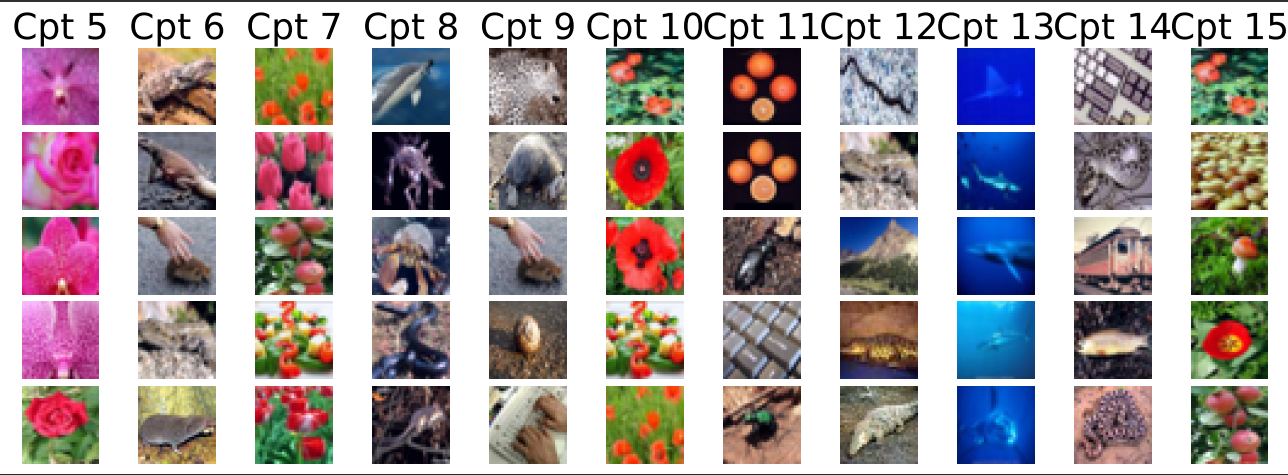
\includegraphics[width=1.0\columnwidth]{images/CGAN_19_32_10_1_cifar100.png}
    \caption{Top 5 images for CIFAR100 that activate the learnt concepts (10 concepts from a subset of 100) using cGAN (VGG 19) DAN  (B=32, S=10). Eg: Cpt 5 corresponds to color pink, Cpt 13 corresponds to object in ocean.}
    \label{fig:cgan_19_cifar100}
\end{figure}

\begin{figure}
    \centering
    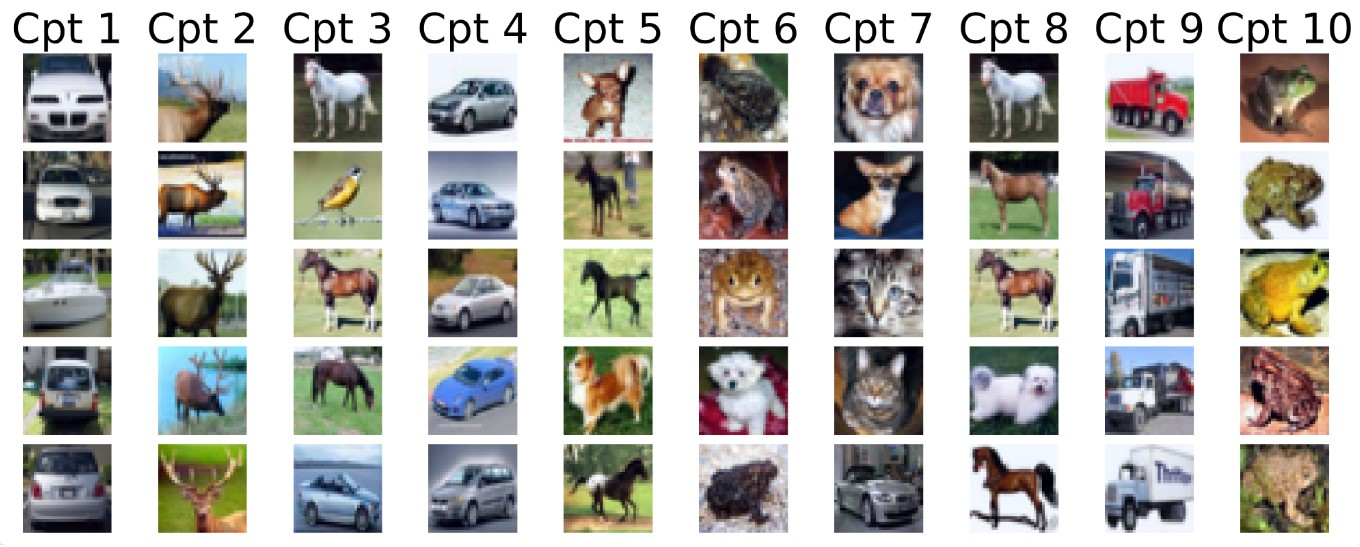
\includegraphics[width=1.0\columnwidth]{images/cgan11.jpg}
    \caption{Top 5 images for CIFAR10 that activate the learnt concepts using cGAN (VGG 11) DAN  (B=32, S=10). Eg: Cpt 2 captures antlers, Cpt 1 captures the color white - here we see that activated images are from different classes (ship, car).}
    \label{fig:cgan11}
\end{figure}

\subsection{Observations}\label{sec:observations}
The preceding sections discussed how various VGG models can influence the performance of our framework. Our observations underline that GAN-based conditioning, cGAN, introduces notable improvements. 
%This results from the conditioning's inherent capacity to control image generation, thereby enhancing the model's predictive outcomes.
A general trend observed indicates that VGG model depth correlates with improved performance, particularly in terms of accuracy. 
%Our study reveals that among the methods, DAN coupled with cGAN and VGG 19 yields the most favourable results with an accuracy of \textbf{91.82\%}. 
%Additionally, in many instances, the alternative methods perform similar to \cite{Sarkar2021AFF} when comparing the Accuracy.
We also see that a correlation between dataset scale and auxiliary accuracy, from the fact that our method consistently gives better auxiliary accuracy compared to the baselines on CIFAR100.

Another significant observation is that the increasing complexity of the model due to the GAN integration and noise sampling methodologies (as detailed in Section \ref{sec:data_noise} of appendix); increase training time by 1.4 times that of \cite{Sarkar2021AFF}. Despite this, the training efficiency remains considerably superior to that of SENN.





\section{Conclusion and Future Work}\label{sec:conclusion}
In conclusion, this work presents a method for incorporating a Generative Adversarial Network (GAN) into an ante-hoc explainability framework. The design replaces a conventional decoder network with a GAN and fine-tunes the framework. The exploration of noise sampling methods, specifically the implementation of DAN, demonstrate superior performance, proving the effectiveness of a GAN in aiding the process of encoding concepts. 
We have observed results that signify an improved overall accuracy and auxiliary accuracy, highlighting the potential of our architecture for robust image classification and effective concept learning. 
%We also observe a positive correlation between the size of the VGG network in the discriminator and the accuracy achieved could guide future architectural choices.  

Although, we have made some improvements on enhancing the explainability of deep neural networks without losing out on classification performance, the work presented is a small step towards a much more robust and human interpretable model.
%In the past, such Deep Neural Network models did not have the capability to explain their predictions, whereas now the field has seen a lot of advancements. 
In the future, we plan on exploring the possibilities of more advanced and complex architectures that could involve using a much deeper classification models such as ResNet, EfficientNet, Mask RCNN. We also plan on making use of the capabilities of some state-of-the-art architectures such as Vision Transformers in conjunction with our framework. Another empirical observation we made is that different noise methods work well for different configurations. We plan on further analysis along this direction.


% \bibliographystyle{aaai24}
\bibliography{aaai24}

\appendix
% \tableofcontents
% \etocdepthtag.toc{mtappendix}
% \etocsettagdepth{mtchapter}{none}
% \etocsettagdepth{mtappendix}{subsection}
% \tableofcontents
% \localtableofcontents
\section{Appendix}
\subsection{Acknowledgements}
We would like to thank the authors of \cite{Sarkar2021AFF} for their guidance and insighful discussions. We would also like to thank the anonymous reviewers for their valuable feedback.
% \localtableofcontents
\subsection{Related Work}\label{sec:rel_work}

\textbf{Post-Hoc Methods:} In addition to Saliency Maps \cite{saliency_maps} and Grad-CAM \cite{GradCAM}, other influential post-hoc techniques include LIME \cite{guestrin} and DeepLift \cite{deeplift}. LIME provides model-agnostic local explanations by approximating any classifier with an interpretable linear model. DeepLift decomposes the predictions of a Deep Neural Network by backpropagating contribution scores to the inputs. Most of these methods are gradient-based, with the problem of the root cause  of errors being difficult to diagnose.


\textbf{Concept-based Models: }\cite{CBM} propose concept bottleneck models with a concept layer to improve interpretability and enable test-time human intervention. These models are trained on both task labels and user-specified concepts via a two-step process where inputs predict concepts and concepts predict labels. This interpretable structure allows for interventions, where experts can correct wrong predictions by modifying concept values, enabling model interaction. However, intervention effectiveness depends on the training approach, highlighting the need to study factors beyond just accuracy. While subsequent works expanded these ideas \cite{interactive, zarlenga2022concept, yuksekgonul2022posthoc}, there has been some criticism as to whether these models truly learn as intended \cite{margeloiu2021concept}.

\textbf{Prototype-based Learning: }\cite{prototype_paper} introduce an approach for interpreting deep neural networks by integrating an autoencoder with a \textit{prototype} layer during training. The model classifies inputs based on their proximity to encoded examples in the prototype layer, facilitating an intuitive case-based reasoning mechanism. The jointly optimized prototypes, guided by various loss terms, connect the network's decisions with explanations, visible through visualization of class-representative prototypes. While achieving competitive accuracy compared to CNN baselines, the method offers integrated explanations without post-hoc techniques. 
Several extensions to prototype-based methods have been proposed, like \cite{prototype_1, Donnelly_2022_CVPR}

\textbf{Other methods: } Several prior studies have developed methods focusing on both high accuracy and explainability. Some methods take the approach of making use of auto-encoders that could enable the reconstruction of images such as \cite{efros2}. There human-in-the-loop works related to involving human feedback and developing concepts that both align with human's intuition of concept such as \cite{concept_human}. Several derivatives of prototype-based models have proven to be quite impressive at visualizing representations and explanations \cite{prototype}.

\subsection{Implementation Details}
All our experiments were conducted on NVIDIA GeForce GTX 1080 Ti. The generator architecture comprises multiple deconvolution layers, generating images using learned concepts and noise, and incorporating labels in the case of cGAN. The discriminator architecture has a VGG network backbone with few additional layers to re-purpose it into a binary classifier. We have tested with different VGG \cite{VGG} architectures such as VGG 8, VGG 11 and VGG 19. 


\subsection{Datasets and Comparison Methods}\label{sec:data_noise}

\textbf{Datasets}: For our experiments, we choose the CIFAR-10 and CIFAR-100 \cite{CIFAR10} benchmarks to facilitate comparisons with prior work. CIFAR-10 consists of 60,000 32x32 coloured images from 10 classes, with 6,000 images per class. The dataset split of 50,000/10,000 train/test images providing sufficient data for training deep networks while maintaining a separate test set for unbiased evaluation. CIFAR-100 is slightly more challenging, containing the same number of images but partitioning them into 100 classes, each with 600 images. This increased class variability and lower samples per class simulate real-world fine-grained classification challenges more closely. Compared to CIFAR-10, CIFAR-100 tests a model's ability to discriminate between subtle inter-class differences.


We chose CIFAR-10 and CIFAR-100 as their moderate sizes allowed us to conduct extensive experiments in reasonable time to thoroughly test different architectures and design decisions, as compared to huge datasets such as ImageNet \cite{IMAGENET}. Both the datasets contain complex and diverse real life objects in various backgrounds. 

\textbf{Noise Methods}: This study introduces a framework with an emphasis on the integration of noise into the network, typically drawn from a Normal distribution $\mathcal{N}(0,1)$. The impact of various noise sampling techniques on GAN training has been thoroughly studied. Given the batch size $B$ of images as 32, concepts of size 10, and a designated noise size $S$ of 5, the shape of the concepts and the noise would be \texttt{32x10x1} (\(B \times C \times 1\)) and \texttt{32x5x1} (\(B \times S \times 1\)), respectively. Once the noise is added, the final shape of the concepts would be \texttt{32x15x1} (\(B \times (C+S) \times 1\)). Different noise generation strategies are explored. The noise sampled helped us in determining the effects of different noise perturbations on our model.

\textbf{Method 1: Direct Align Noise (DAN):} The noise is directly aligned with batch size and noise length. Consequently, the sampled noise follows the shape (\(B \times S \times 1\)) where the entire (\(B \times S \times 1\)) matrix is sampled from $\mathcal{N}(0,1)$ and together represents a Gaussian.

\textbf{Method 2: Iterative Concat Noise (ICN):} The noise is sampled multiple times to achieve the desired dimension. Initially, noise is sampled as \(B \times 1 \times 1\) and then concatenated \(S\) times. Each row of size \(B \times 1 \times 1\) is sampled from a Gaussian.

\textbf{Method 3: Progressive Concat Noise (PCN):} The noise is sampled multiple times, but it begins with an even smaller dimension. Noise is initially sampled as \(1 \times S \times 1\) and then concatenated \(B\) times. Each column of size \(1 \times S \times 1\) is sampled from a Gaussian.


%This assortment of noise sampling techniques allows adaptability, enhancing image quality and overall model efficiency. These strategies are pivotal for tuning noise components to meet diverse requirements, ultimately elevating the quality of generated images and contributing to the GAN architecture's effectiveness. 
We show that introducing noise improves model adaptability, enhancing image quality and overall model efficiency.
One point to note is that the ICN and PCN vectors, when concatenated may not represent a Gaussian. Our framework can be extended to incorporate other noise methods as well.
 

\begin{table*}[h!]
\scalebox{0.9}{
\begin{tabular}{c|c|cc|cc|cc}
\toprule
\multirow{2}{*}{Model}   & \multirow{2}{*}{VGG Model} & \multicolumn{2}{c}{DAN} & \multicolumn{2}{c}{ICN} & \multicolumn{2}{c}{PCN} \\ 
 &
   &
  \multicolumn{1}{c}{Accuracy} &
  \multicolumn{1}{c|}{Aux. Accuracy} &
  \multicolumn{1}{c}{Accuracy} &
  \multicolumn{1}{c|}{Aux. Accuracy} &
  \multicolumn{1}{c}{Accuracy} &
  \multicolumn{1}{c}{Aux. Accuracy} \\ \midrule
\multicolumn{1}{c|}{cGAN (B=32, S=10)} &
  \multicolumn{1}{c|}{11} &
  \multicolumn{1}{c}{\textbf{65.37}} &
  \multicolumn{1}{c|}{45.36} &
  \multicolumn{1}{c}{65.15} &
  \multicolumn{1}{c|}{41.69} &
  \multicolumn{1}{c}{65.21} &
  \multicolumn{1}{c}{{45.44}} \\ 
\multicolumn{1}{c|}{cGAN (B=32, S=10)} &
  \multicolumn{1}{c|}{19} &
  \multicolumn{1}{c}{\textbf{64.42}} &
  \multicolumn{1}{c|}{{44.92}} &
  \multicolumn{1}{c}{62.42} &
  \multicolumn{1}{c|}{44.87} &
  \multicolumn{1}{c}{64.00} &
  \multicolumn{1}{c}{44.56} \\ 
\multicolumn{1}{c|}{Vanilla GAN (B=32, S=10)} &
  \multicolumn{1}{c|}{11} &
  \multicolumn{1}{c}{\textbf{65.49}} &
  \multicolumn{1}{c|}{45.05} &
  \multicolumn{1}{c}{65.13} &
  \multicolumn{1}{c|}{46.16} &
  \multicolumn{1}{c}{65.47} &
  \multicolumn{1}{c}{{45.80}} \\ 
Vanilla GAN (B=32, S=10) & 19                         & \textbf{60.71}      & 44.52      & 58.09      & 43.78      & 60.02      & {46.19}      \\ \bottomrule
\end{tabular}
}
\caption{\textit{Accuracy} (in \%) and \textit{Auxiliary Accuracy} in (\%) for comparing our models on CIFAR100. cGAN = Conditional GAN, B = Batch Size, S = size of Noise. Aux. Accuracy = Auxiliary Accuracy. We see that different noise methods work well on different models. We are choosing the best noise method.}
\label{tab:cifar100_compare}
\end{table*}


\begin{table*}[ht!]
\centering
\scalebox{0.91}{
\begin{tabular}{c|c|cc|cc|cc}
\toprule
\multirow{2}{*}{Model} &
  \multirow{2}{*}{VGG Model} &
  \multicolumn{2}{c}{DAN} &
  \multicolumn{2}{c}{ICN} &
  \multicolumn{2}{c}{PCN} \\
 &
   &
  \multicolumn{1}{c}{Accuracy} &
  Aux. Accuracy &
  \multicolumn{1}{c}{Accuracy} &
  Aux. Accuracy &
  \multicolumn{1}{c}{Accuracy} &
  Aux. Accuracy \\ \midrule
Vanilla GAN  (B=32, S=10) & 8  & \multicolumn{1}{c}{91.53} & 90.00    & \multicolumn{1}{c}{\textbf{91.57}} & 89.63 & \multicolumn{1}{c}{91.41} & 89.57 \\
Vanilla GAN  (B=32, S=10) & 11 & \multicolumn{1}{c}{91.38} & 89.63 & \multicolumn{1}{c}{90.80}  & 89.37 & \multicolumn{1}{c}{\textbf{91.66}} & 90.94 \\ 
cGAN  (B=32, S=10)        & 8  & \multicolumn{1}{c}{91.55} & 90.15 & \multicolumn{1}{c}{91.44} & 90.13 & \multicolumn{1}{c}{\textbf{91.60}}  & 89.94 \\ 
cGAN (B=32, S=10)         & 11 & \multicolumn{1}{c}{\textbf{91.58}} & 89.90  & \multicolumn{1}{c}{91.34} & 89.96 & \multicolumn{1}{c}{91.28} & 89.82 \\ 
cGAN (B=32, S=5)          & 11 & \multicolumn{1}{c}{91.36} & 89.74 & \multicolumn{1}{c}{91.44} & 89.77 & \multicolumn{1}{c}{\textbf{91.47}} & 89.68 \\ 
cGAN (B=32, S=10)         & 19 & \multicolumn{1}{c}{91.52} & 90.09 & \multicolumn{1}{c}{\textbf{91.76}} & 90.08 & \multicolumn{1}{c}{91.45} & 89.99 \\ 
cGAN (B=32, S=5)          & 19 & \multicolumn{1}{c}{\textbf{91.82}} & 90.23 & \multicolumn{1}{c}{91.15} & 89.62 & \multicolumn{1}{c}{91.44} & 89.60  \\ \bottomrule
\end{tabular}}
\caption{\textit{Accuracy} (in \%) and \textit{Auxiliary Accuracy} in (\%) for comparing our models on CIFAR10. cGAN = Conditional GAN, B = Batch Size, S = size of Noise. Aux. Accuracy = Auxiliary Accuracy. We see that different noise methods work well on different models.}
\label{tab:all_model}
\end{table*}




\subsection{Additional Results}\label{sec:add_results}
This section displays additional concept visualization results that could not be included in the main paper. These results are based on CIFAR10 as well as CIFAR100 for both Vanilla GAN and Conditional GAN.

We also perform comparative analysis on different noise methods (discussed in Section \ref{sec:data_noise}) on our framework with different VGG models and both Vanilla GAN and Conditional GAN.

\textbf{Vanilla GAN:}\label{sec:van_gan} 
%In the context of Vanilla GAN, we will differentiate between different discriminator architectures and choose the best model out each of the architectures with respect to the noise methods.
As shown in Table \ref{tab:all_model}, in the case of \textbf{CIFAR10}, for VGG 8, we observe that ICN  gives the best accuracy of \textbf{91.57\%}. While in the case of VGG 11, PCN  gives better results, with an accuracy of \textbf{91.66\%}. 
As shown in Table \ref{tab:cifar100_compare}, on \textbf{CIFAR100}, for VGG 11 we observe that DAN  has the best accuracy of \textbf{65.49\%}. DAN  also gives the best accuracy of \textbf{60.71\%} for VGG 19.
%While in the case of VGG 19, DAN (Method 1) has a better accuracy of as compared to other methods.



\begin{figure}[h!]
    \centering
    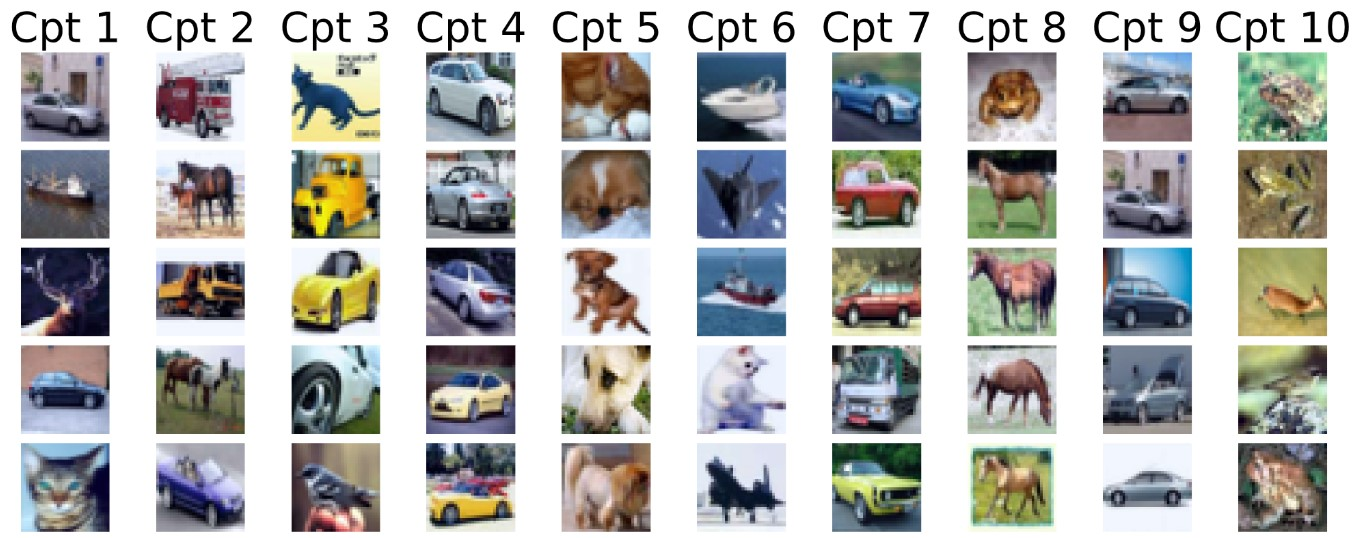
\includegraphics[width=1.0\columnwidth]{images/cgan19.jpg}
    \caption{Top 5 images for CIFAR10 that activate the learnt concepts using cGAN (VGG 19) DAN (B=32, S=5). Eg: Cpt 9 captures a concept corresponding to the grey color, Cpt 10 corresponds to frog skin.}
    \label{fig:cgan19}
\end{figure}

\begin{figure}[h!]
    \centering
    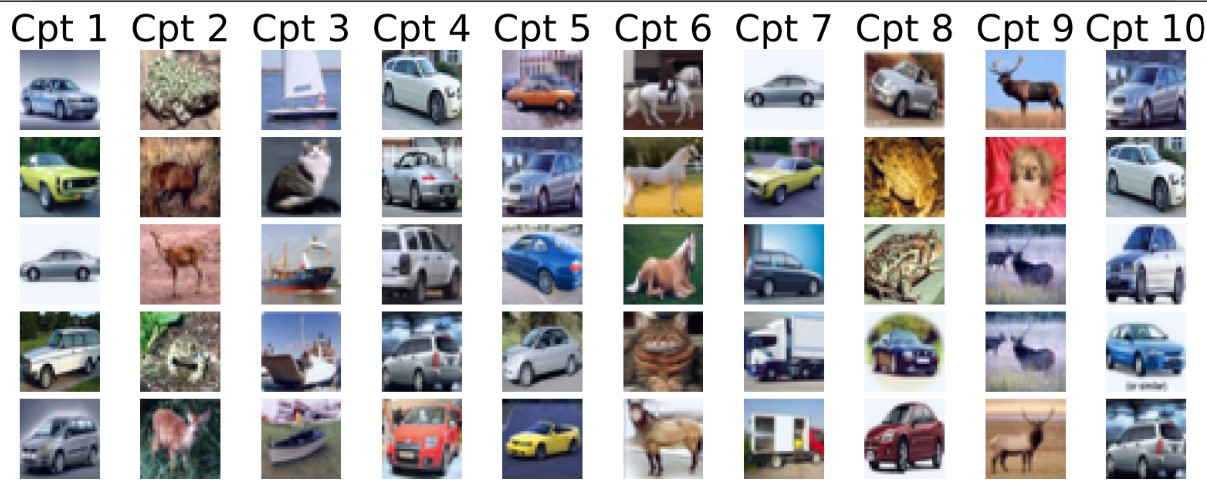
\includegraphics[width=1.0\columnwidth]{images/vcan8.jpg}
    \caption{Top 5 images for CIFAR10 that activate the learnt concepts using Vanilla GAN (VGG 8) ICN  (B=32, S=10). Eg: Cpt 9 corresponds to antlers, Cpt 6 corresponds to shape of legs.}
    \label{fig:vgan8}
\end{figure}

\begin{figure}[h!]
    \centering
    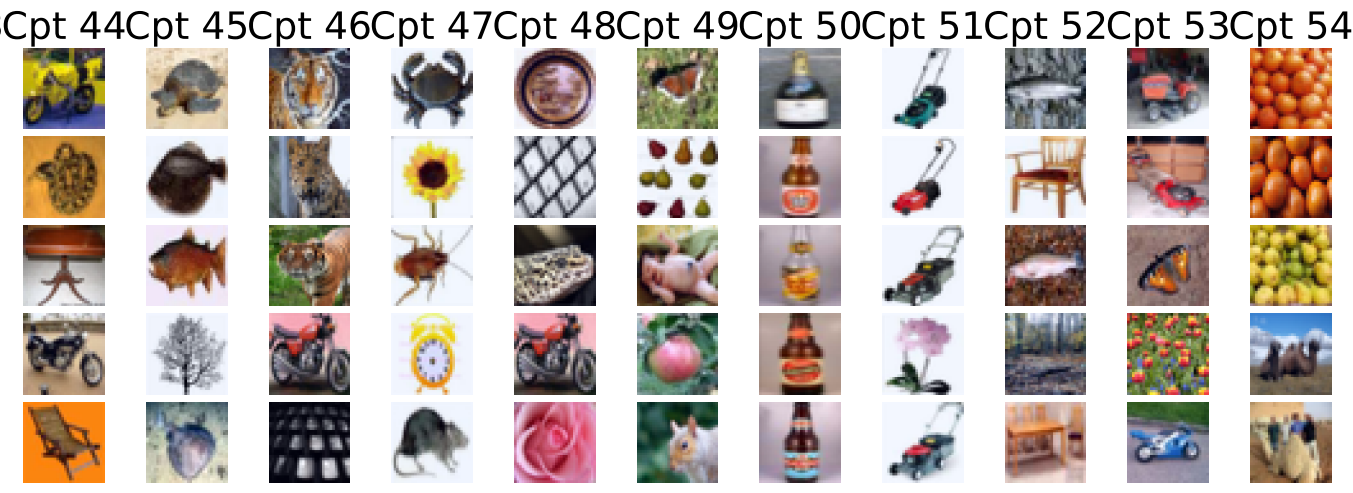
\includegraphics[width=1.0\columnwidth]{images/CGAN_11_1_10_1_cifar100.png}
    \caption{Top 5 images for CIFAR100 that activate the learnt concepts (10 concepts from a subset of 100) using cGAN (VGG 11) PCN  (B=32, S=10). Eg: Cpt 50 corresponds to shape of a bottle, and Cpt 51 corresponds to a lawn-mower.}
    \label{fig:cgan_11_cifar100}
\end{figure}

\begin{figure}[h!]
    \centering
    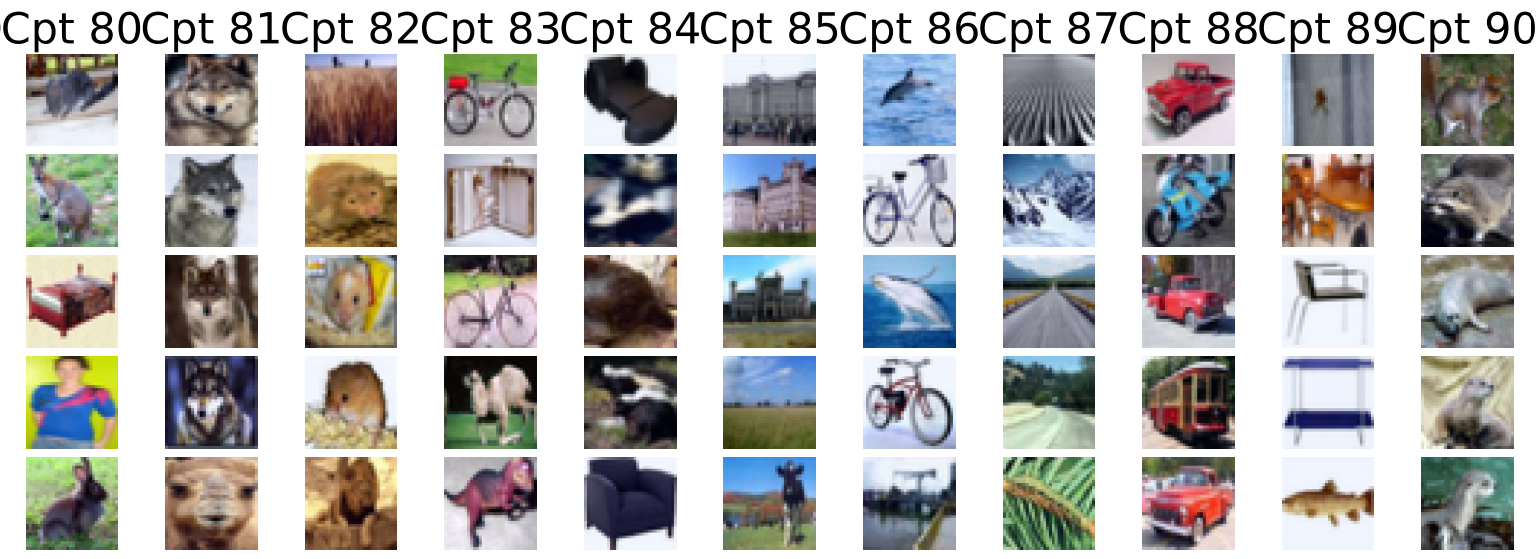
\includegraphics[width=1.0\columnwidth]{images/GAN_11_32_10_1_cifar100.png}
    \caption{Top 5 images for CIFAR100 that activate the learnt concepts (10 concepts from a subset of 100) using Vanilla GAN (VGG 11) DAN (B=32, S=10). Eg: Cpt 81 corresponds to face of a wolf, Cpt 88 corresponds to wheels.}
    \label{fig:cgan_11_cifar100}
\end{figure}

\textbf{cGAN:}\label{sec:cond_gan}
%In the context of cGAN, we will differentiate between different discriminator architectures and choose the best model out each of the architectures with respect to the noise methods. 
Here, in addition to a noise size of 10, we also experiment with a noise size of 5 to examine its effect on the framework.
As shown in Table \ref{tab:all_model}, for \textbf{CIFAR10}, using VGG 8, PCN gives the best accuracy of \textbf{91.60\%}. In the case of VGG 11, for a noise size of 10, we get better results using DAN - with an accuracy of \textbf{91.58\%}; whereas for a noise size of 5, we get better results using PCN - with an accuracy of \textbf{91.47\%}. Finally, in the case of VGG 19, DAN gives the best results when using a noise size of 5.
As shown in Table \ref{tab:cifar100_compare}, for \textbf{CIFAR100}, we consistently observe that DAN gives the best results. In the case of VGG 11, using DAN we get the best accuracy of \textbf{65.37\%}. With VGG 19, using DAN we get the best accuracy of \textbf{64.42\%}.

% \subsection{Reviewer Answers}
% For CIFAR100, Our model takes approximately, 0.52 sec for each batch and a total average of 12 minutes for each epoch. In order to compare with our model, \cite{Sarkar2021AFF} took 0.26 sec for each batch and a total average of 6 min for each epoch. \cite{SENN} took 0.84 sec for each batch and a total average of 20 min for each epoch. The model complexity increases significantly with the addition of a GAN and VGG network as discriminator. The improvement is marginal, but the computational time is not significantly larger as compared to \cite{SENN}.

% The main task of our research was to study the how an adversarial nature could be incorporated in an ante-hoc concept learning framework and also study the effects of different noise sampling techniques on the robustness of the framework. Our results seem to be a marginal increase over our baseline, but our empirical study indicates that we can incorporate a generative model into such a framework and receive an improvement in the learning of concepts.

% The noise sampling methods were introduced to study how noise fed into a generator with concepts to generate images that could train the encoder to encode relevant concepts that could be human-interpretable.

% \cite{Sarkar2021AFF} used a simple decoder and L-2 distance loss function to implement and test their theory. We wanted to increase the model complexity to capture richer concepts, as well as improve performance by using a GAN. The adversarial nature of GAN impacts the encoder during the training process. This helps capture more explainable concepts that could be visualized in the figures. 
% The discriminator would allow the generated image to represent the original image as close as possible. Moreover, conditioning the GAN over labels additionally helps the network learn better concepts that can be visualized in the figures.

% Increasing the model complexity helps us capture richer concepts that can be validated from the figures. The adversarial nature of GANs impact the encoder during the training process making it capture more explainable concepts.

\end{document}